% !TeX spellcheck = en_GB
\begin{figure}[t]
	\centering
	\begin{subfigure}[b]{0.32\textwidth}
		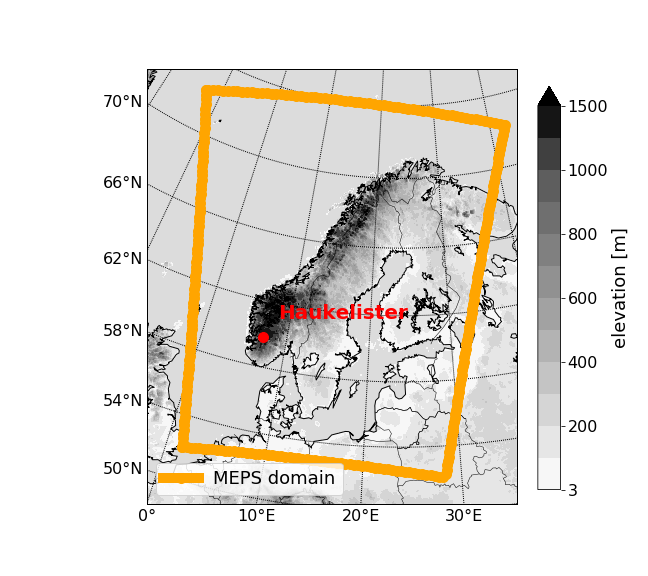
\includegraphics[trim={2.75cm 1.8cm 4.4cm 2.3cm},clip,
		width=\textwidth]{./fig_Norway/Norway_MEPS}
		\caption{}\label{fig:site:Norway}
	\end{subfigure}
	%%%%% zoomed in map
	\begin{subfigure}[b]{0.32\textwidth}
		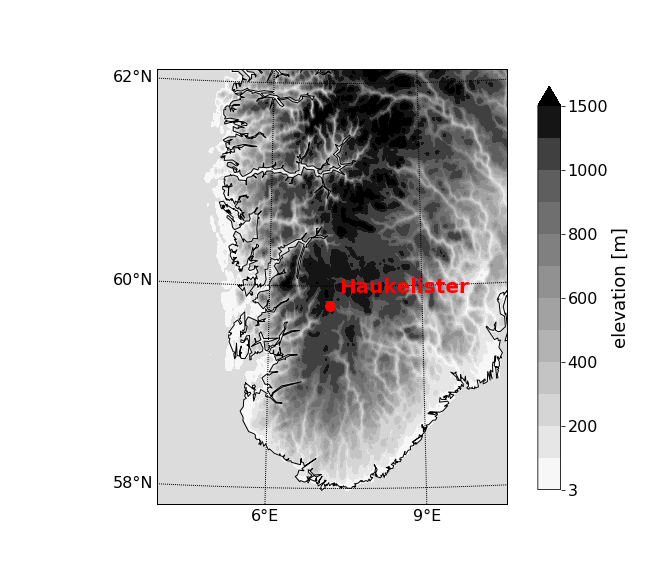
\includegraphics[trim={2.75cm 1.8cm .65cm 2.3cm},clip,
		width=\textwidth]{./fig_Norway/South_Norway}
		\caption{}\label{fig:site:Nzoom}
	\end{subfigure}
	%%%%% zoomed in kartverketmap
	\begin{subfigure}[b]{0.32\textwidth}
		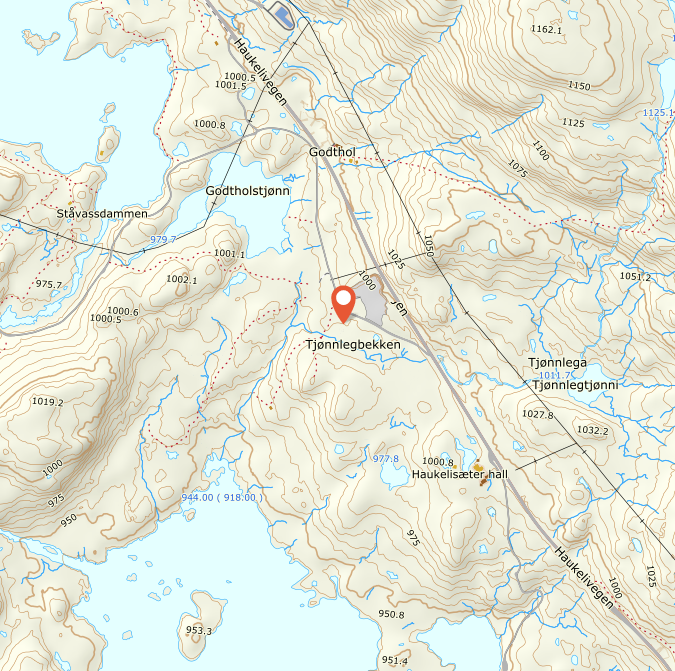
\includegraphics[width=\textwidth]{./fig_Norway/Haukeli_site}
		\caption{}\label{fig:site:kartverket}
	\end{subfigure}
	\caption{Elevation map of Northern Europe (\protect\subref{fig:site:Norway}) and South Norway (\protect\subref{fig:site:Nzoom}). Red dot indicates the location Haukeliseter and the orange square in \subref{fig:site:Norway} indicates the model domain of MEPS. Elevation according to the shading. \protect\subref{fig:site:kartverket}: topographical map of the measurement site marked with a red pin \citep{kartverket_norgeskart_2018}.} \label{fig:site}
\end{figure}